\documentclass{scrartcl}

\usepackage{graphicx}

\usepackage{caption}
\usepackage{subcaption}

\usepackage{microtype}
\usepackage[inkscapeformat=eps, inkscapepath=svgdir]{svg}

\usepackage{amsmath}
\usepackage{amssymb}

\usepackage[style=ieee]{biblatex}
\usepackage{hyperref}
\usepackage{cleveref}

\addbibresource{main.bib}

\title{Advanced Data Analysis and Machine Learning - Practical Activities}
\subtitle{Semi-Supervised Learning}
\author{Sergio Mauricio Vanegas Arias}
\date{\today}

\begin{document}

\maketitle

\section{Introduction}

  This week, we were asked to experiment with Transfer Learning, taking a pre-trained object-detection model and fine-tuning it to recognize 4 letters of the sign language (G,H,K,M). The given dataset was intentionally tainted with to increase the training task, and the objective is to be able to correctly classify our own photos of sign language.

  The specific tasks were the following:
  \begin{enumerate}
    \item Visualize the dataset and identify its problems
    \item Present the architecture of the pre-trained model and the data it has been trained on
    \item Propose an augmentation strategy and explain the necessity to implement one
    \item Train the model for the specific task
    \item Evaluate the importance of augmentation steps\footnote{This was done at the same time as the augmentation strategy proposal}
    \item Test the model with our own data\footnote{Unfortunately, I did not have time to test the fine-tuned model on my own images, but the code to unlock the base model and perform further optimization can be found in the attached notebook}
  \end{enumerate}

\section{Dataset Visualization}

  \begin{figure}[ht]
    \centering
    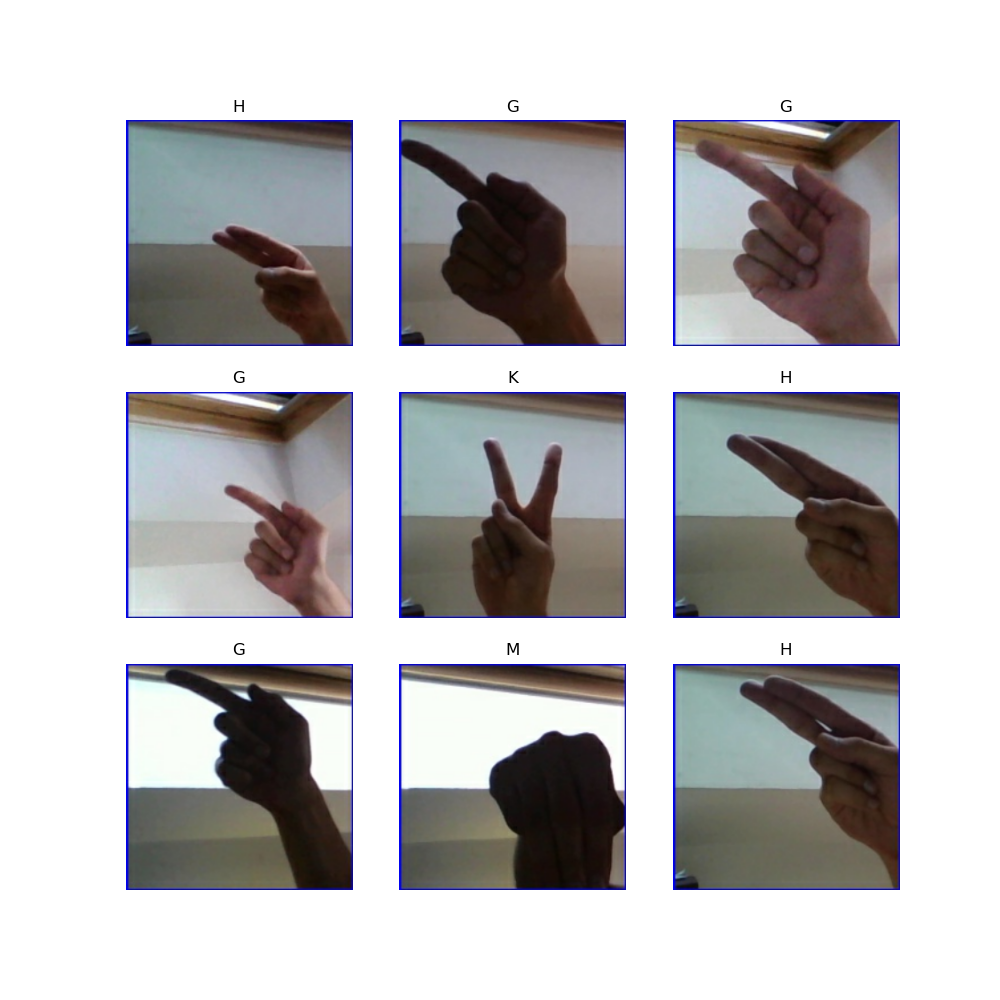
\includegraphics[width=0.75\textwidth]{../figures/rgb_overview.png}
    \caption{Original dataset visualization}
    \label{fig:rgb_overview}
  \end{figure}

  \Cref{fig:rgb_overview} shows the original dataset, with a sample count of $68/48/30/41$ for the classes G/H/K/M respectively. Besides the clear class imbalance, there were also focus and contrast problems with the given images, which results in key information not being present in the frame.
  
  Fortunately, by taking a pre-trained convolutional model and then fine-tuning it for our application, the most relevant features can be extracted from relatively little information and a rather small dataset. As for the class imbalance, this can be numerically addressed using class weighting as $$w_i = \frac{N}{C \cdot N_i} ,$$ where $w_i$ is the weight of each class, $N$ is the total number of samples, $C$ is a normalization factor equal to the number of classes, and $N_i$ is the number of samples belonging to the class being weighed.

\section{Pre-trained Model Architecture}

  \begin{figure}[ht]
    \centering
    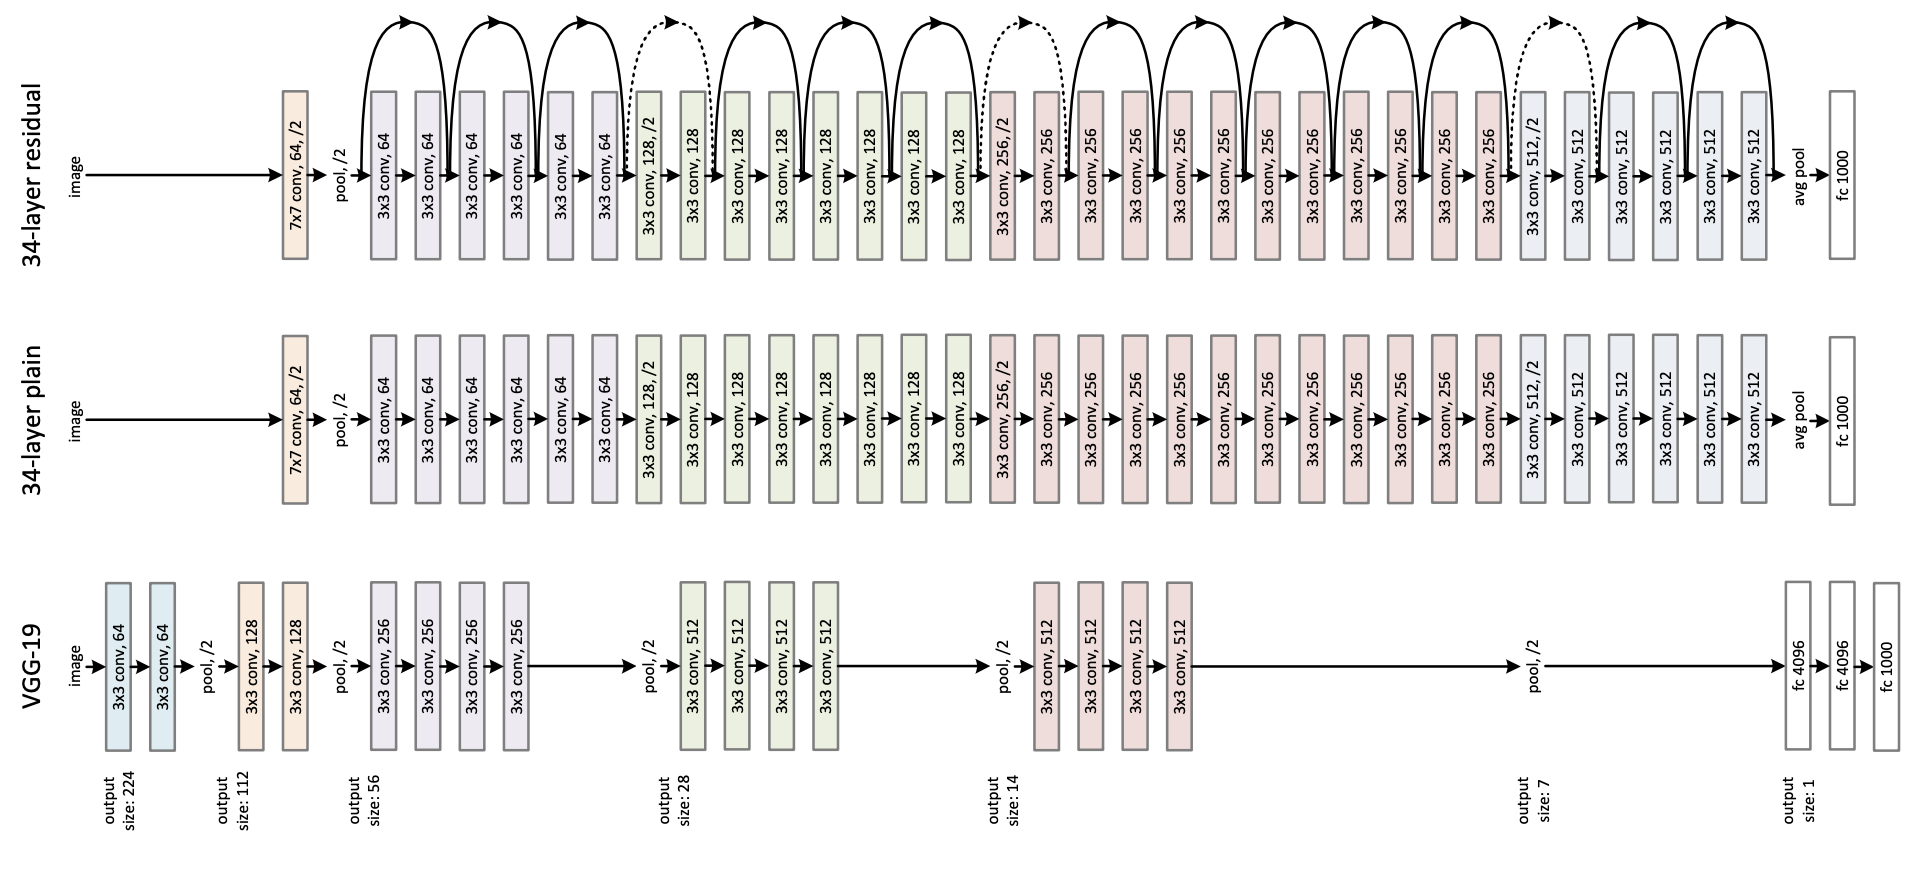
\includegraphics[width=\textwidth]{../figures/base_model.png}
    \caption{Resnet-34 vs 34-layer Plain-network vs VGG-19}
    \label{fig:base_model}
  \end{figure}

  The chosen architecture was a \emph{Deep Residual Convolutional Network} \autocite{he2015deep}; specifically, the Tensorflow/Keras implementation of Resnet-152\footnote{The smaller resnet-34 is shown in \Cref{fig:base_model} instead due to the model's size}, which was originally trained with the general-purpose ImageNet 2012 classification dataset (1000 classes, 1.28 Million training images, 50 Thousand validation images). The reasoning for this was to get as much pre-training as possible in a well-established ML framework that facilitated Transfer Learning with a custom dataset, providing utilities for dataset creation, data augmentation, and parameter locking.

\section{Data Augmentation}

  As mentioned earlier, Transfer Learning enables complex model training from a relatively low sample-size; nevertheless, ML models (particularly in the field of Computer Vision) benefit from larger representative datasets. Thus, by applying sensible (i.e., coherent with reality) data augmentation techniques to the training partition, greater accuracy can be almost effortlessly attained.

  A simple 3-step random augmentation (Zoom, Rotation, and Translation) pipeline is thus applied to the training/validation subsets, thus preserving the ratio used for generating the class weights. These modifications are severely restricted in order to avoid unrealistic hand distortion or semantic changes in the hand gestures. A sample of the output from this pipeline can be observed in \Cref{fig:aug_overview}

  \begin{figure}[ht]
    \centering
    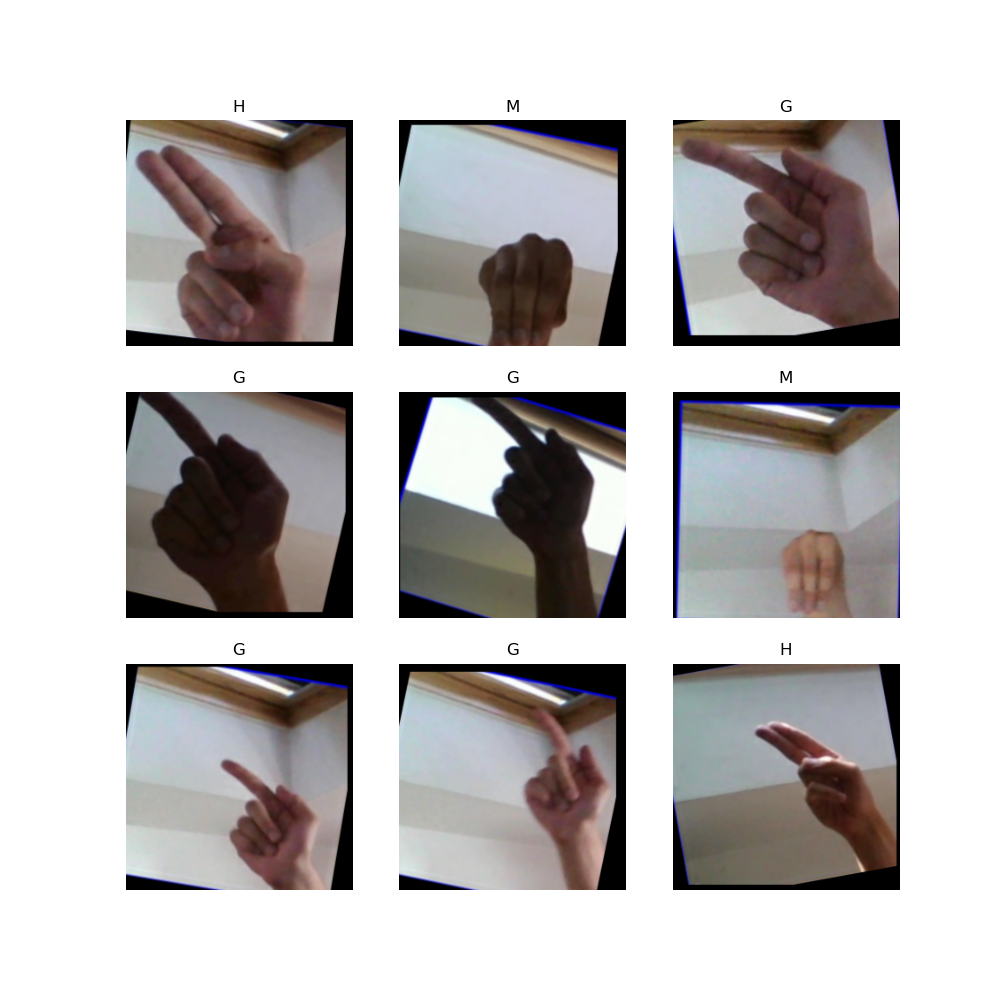
\includegraphics[width=0.75\textwidth]{../figures/aug_overview.png}
    \caption{Augmented dataset visualization}
    \label{fig:aug_overview}
  \end{figure}

\section{Model Training (Practical Considerations)}

  Some practical considerations this time were the following:
  \begin{itemize}
    \item The image pre-processing layer provided by Tensorflow was not serializable, meaning that it could not be stored along with the rest of the model
    \item The original head for the previously mentioned 1000 classes was not imported, adding instead a 4-channel custom output layer for our specific application
    \item Part of the augmented dataset was kept for validation during training in order to avoid overfitting; however, the test partition was kept unmodified for more accurate metrics
  \end{itemize}

  The above resulted in a cross-categorical entropy of 0.8952 and a categorical accuracy of 0.6429 over the test partition. The training history can be observed in \Cref{fig:training_history}, whereas a sample of the model's classification can be found in \Cref{fig:training_results}.

  \begin{figure}[ht]
    \centering
    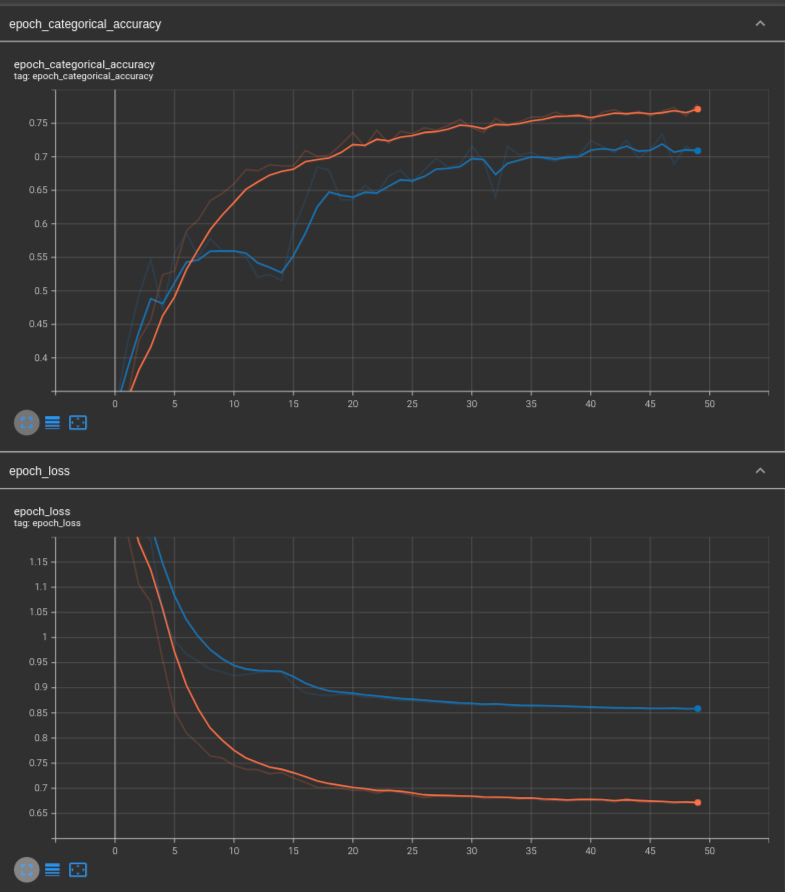
\includegraphics[width=0.75\textwidth]{../figures/training_history.png}
    \caption{Training history}
    \label{fig:training_history}
  \end{figure}

  \begin{figure}[ht]
    \centering
    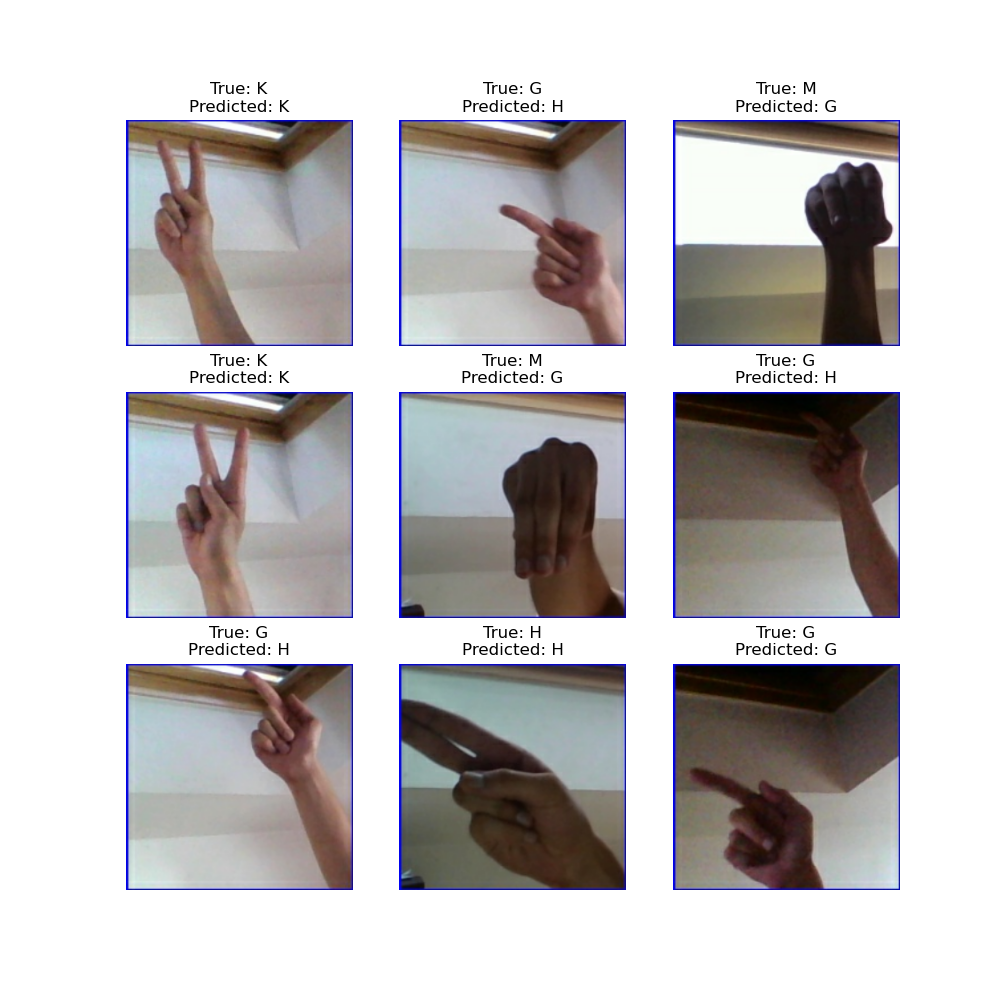
\includegraphics[width=0.75\textwidth]{../figures/trained_model_results.png}
    \caption{Training results}
    \label{fig:training_results}
  \end{figure}

\printbibliography

\end{document}